\chapter{Planificación e seguimento}
\label{chap:planificacion}

Neste capítulo preséntanse a planificación temporal e económica do proxecto, comparando a estimación inicial coa evolución real e analizando as principais desviacións e custos.

\section{Planificación inicial}
De acordo co enfoque incremental descrito no Capítulo \ref{chap:metodoloxia}, o proxecto organizouse en sete incrementos. Cada un deles produciu un resultado concreto sobre o que se puido continuar traballando:

\begin{enumerate}
    \item \textbf{Estudo da viabilidade e investigación de tecnoloxías de extracción automática (15 h):}
    análise das follas de tratamento, identificación da información relevante e estudo das posibles técnicas de visión artificial, recoñecemento óptico de caracteres e procesamento documental.

    \item \textbf{Experimentación e selección da tecnoloxía de extracción (45 h):}
    avaliación das alternativas consideradas e selección da tecnoloxía máis adecuada segundo a calidade da extracción, as súas limitacións e a facilidade de integración.

    \item \textbf{Primeira versión da API (35 h):}
    desenvolvemento dunha proba de concepto capaz de recibir unha folla, invocar o servizo de extracción, procesar o resultado e devolver os datos estruturados.

    \item \textbf{Reorganización da API por capas (20 h):}
    separación dos puntos de entrada, a lóxica de negocio, os modelos de datos e as dependencias externas, incorporando tamén as primeiras probas da API.

    \item \textbf{Primeira versión da aplicación Flutter (100 h):}
    implementación progresiva da configuración inicial, os roles de paciente e supervisor, a persistencia, a incorporación de follas, o calendario e o seguimento das tomas.

    \item \textbf{Integración e estabilización (35 h):}
    conexión da aplicación coa \gls{api} e Firebase, incorporación da vinculación, a sincronización e os recordatorios, e estabilización do sistema mediante probas e corrección de erros.

    \item \textbf{Documentación e entrega (50 h):}
    elaboración e revisión da memoria, dos diagramas e dos materiais necesarios para a entrega e presentación do proxecto.
\end{enumerate}

A planificación inicial comezou o 15 de outubro de 2025 e distribuíu un total de 300 horas entre os sete incrementos descritos anteriormente. Como data interna de finalización do proxecto fixouse o 31 de xullo de 2026, co obxectivo de ter rematados tanto o desenvolvemento como a memoria. A data oficial de entrega mantívose no 11 de setembro de 2026. A planificación temporal completa represéntase no diagrama de Gantt da Figura~\ref{fig:gantt-planificacion-inicial}.

\begin{figure}[h]
    \centering
    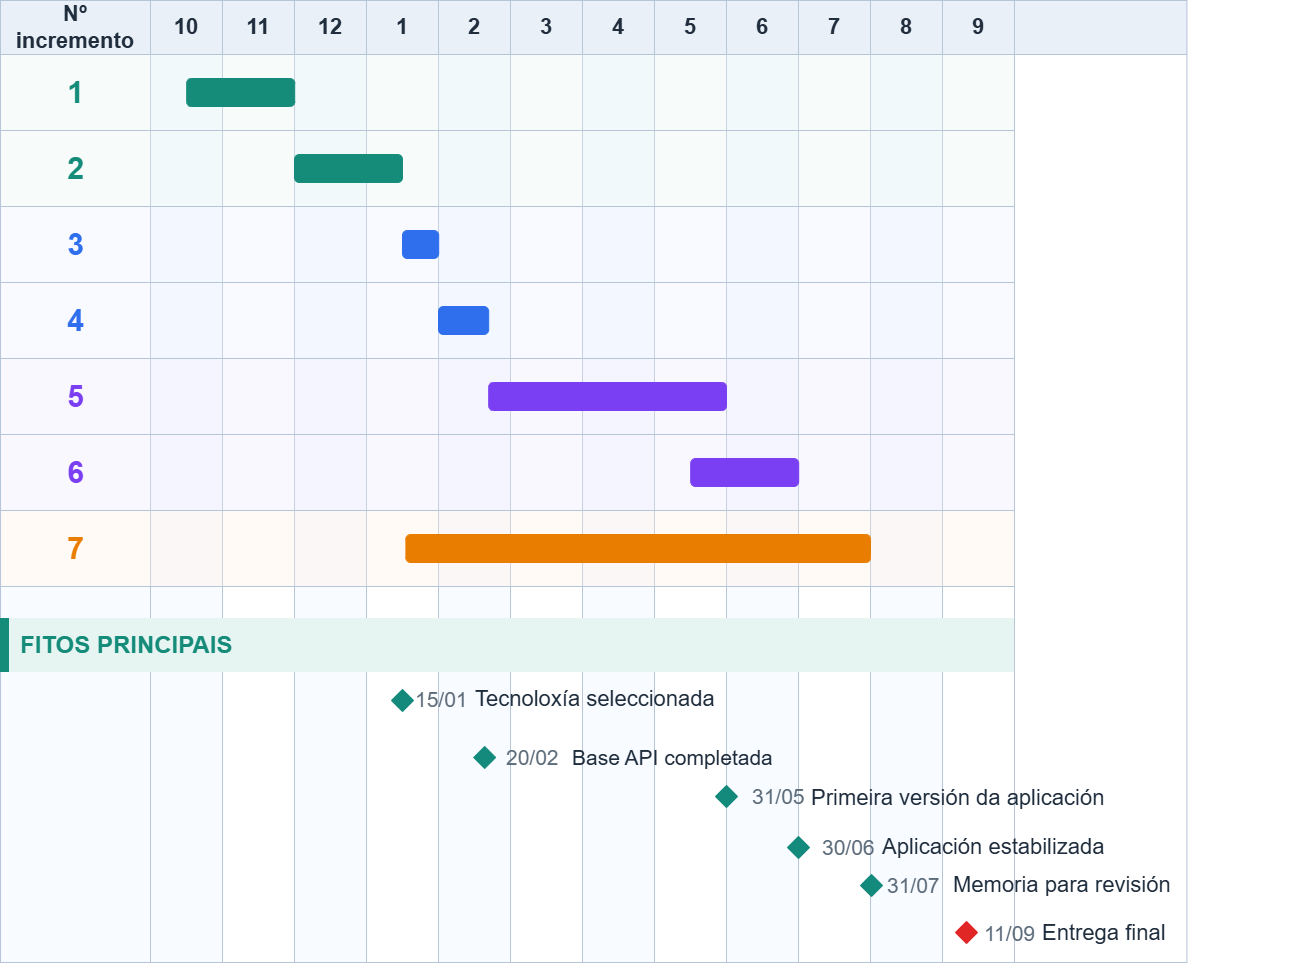
\includegraphics[width=0.75\textwidth]{imaxes/05-Planificacion/gantt-inicial-compacto.drawio.png}
    \caption{Diagrama de Gantt da planificación inicial do proxecto.}
    \label{fig:gantt-planificacion-inicial}
\end{figure}

%ooooooooooooooooooooooooooooooooooooooooooooooooooooooooooooooooooooooooooooooooooooooooooooooooooooo
% HASTA AQUI REVISADO E GUAY
\section{Seguimento e evolución do proxecto}
\label{sec:seguimento-evolucion}

Tal e como se indicou no Capítulo~\ref{chap:metodoloxia}, o control do avance diario levouse a cabo mediante un taboleiro Kanban. Esta xestión visual facilitou o seguimento continuo das tarefas e permitiu adaptar o calendario e a carga de traballo á realidade do desenvolvemento.

Á par desta actualización do calendario, tamén se reavaliou o esforzo necesario. A medida que se avanzaba nas tarefas e se resolvían os primeiros imprevistos, fíxose evidente que a estimación inicial de 300 horas non sería suficiente. Tras revisar a carga de traballo realizada, o historial de confirmacións (\textit{commits}) no repositorio e as métricas do taboleiro Kanban, a dedicación final fixouse nun total de 390 horas (Táboa~\ref{tab:comparacion-horas}). 

\begin{table}[h]
    \centering
    \renewcommand{\arraystretch}{1.2}
    \caption{Comparación entre a dedicación inicial e a dedicación final por incremento.}
    \label{tab:comparacion-horas}
    \small 
    \begin{tabular}{lrrr}
        \toprule
        \textbf{Incremento} &
        \textbf{Inicial (h)} &
        \textbf{Final (h)} &
        \textbf{Diferenza (h)} \\
        \midrule
        Viabilidade e investigación & 15 & 25 & +10 \\
        Experimentación e selección & 45 & 70 & +25 \\
        API inicial & 35 & 45 & +10 \\
        API por capas & 20 & 25 & +5 \\
        Aplicación Flutter & 100 & 125 & +25 \\
        Integración e estabilización & 35 & 50 & +15 \\
        Documentación e entrega & 50 & 50 & 0 \\
        \midrule
        \textbf{Total} & \textbf{300} & \textbf{390} & \textbf{+90} \\
        \bottomrule
    \end{tabular}
\end{table}

Esta cifra supón un incremento de 90 horas, equivalente ao 30\,\% sobre a liña base, e constitúe unha avaliación fundamentada da dedicación real requirida polo proxecto. As causas desta desviación analízanse a continuación.

\subsection{Análise das desviacións}
\label{subsec:analise-desviacions}

A planificación inicial sufriu varias desviacións durante o desenvolvemento. A fase de investigación e experimentación prolongouse pola dificultade para recompilar follas de tratamento e pola necesidade de avaliar distintas tecnoloxías antes de seleccionar unha alternativa fiable. Na \gls{api} foi necesario dedicar máis tempo do previsto ao procesamento e á validación dos datos extraídos, mentres que no cliente móbil a incorporación e revisión de funcionalidades, a integración dos compoñentes e a corrección dos problemas detectados aumentaron tamén a carga de traballo.

A estas desviacións sumouse o cambio na dispoñibilidade horaria. Desde o 17 de marzo de 2026, co inicio das prácticas en empresa, o traballo no proxecto quedou principalmente limitado ás tardes e ás fins de semana e tivo que compaxinarse co resto das materias. Como consecuencia, non se acadou o obxectivo interno de finalizar o proxecto antes do verán, a estabilización prolongouse ata o 15 de agosto e a memoria ata o 31 de agosto, mantendo en todo caso marxe respecto da entrega oficial do 11 de setembro de 2026. O resultado final da planificación móstrase na Figura~\ref{fig:gantt-final}.

\begin{figure}[h]
  \centering
   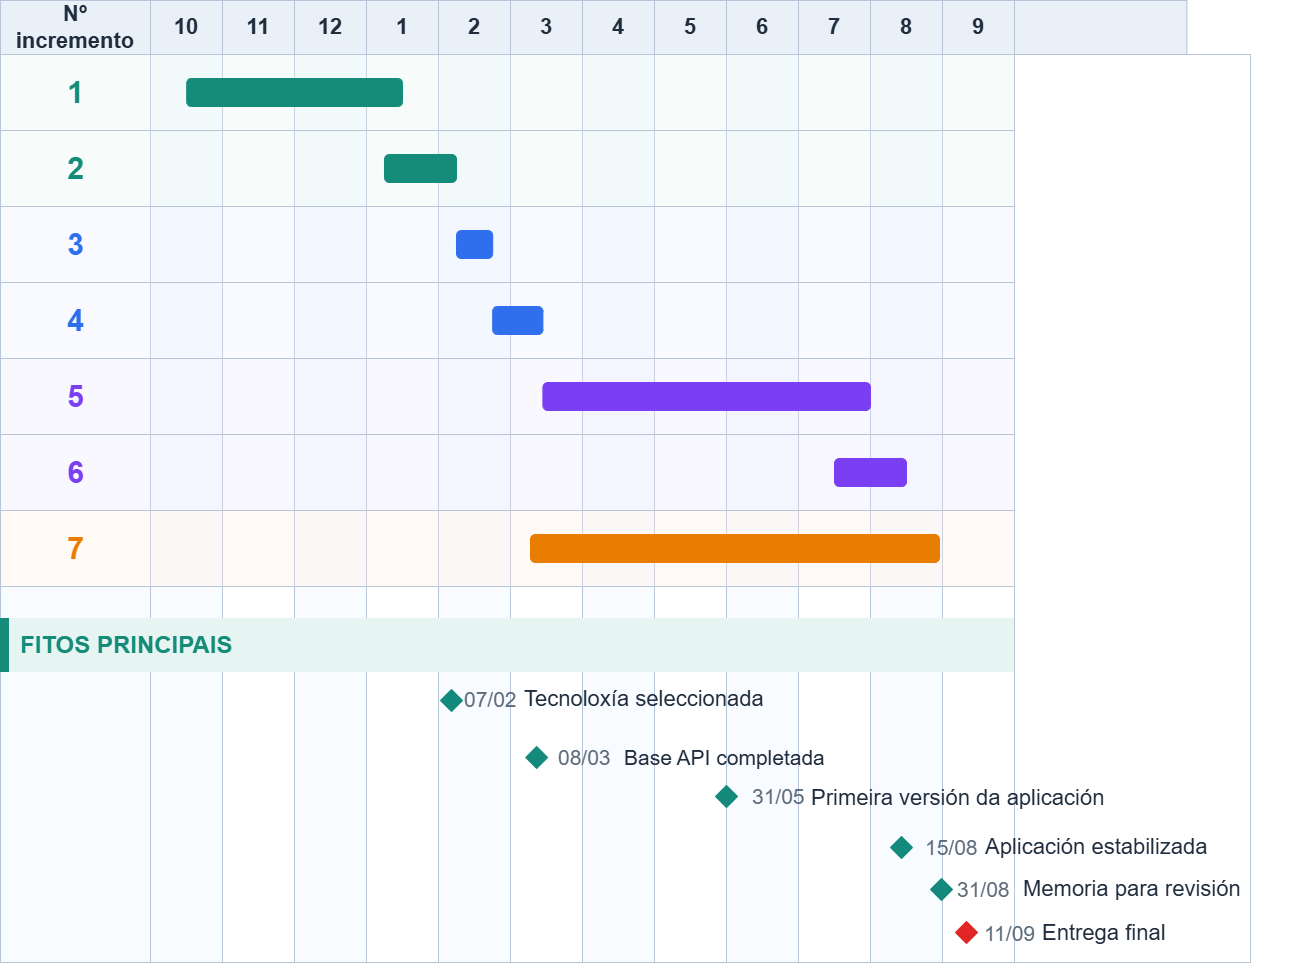
\includegraphics[width=0.75\linewidth]{imaxes/05-Planificacion/gantt-revisado-compacto.drawio.png}
   \caption{Diagrama de Gantt da planificación final do proxecto.}
   \label{fig:gantt-final}
\end{figure}


\section{Custos}
\label{sec:custos-iniciais-revisados}

Para valorar economicamente o esforzo dedicado ao proxecto, tomouse como referencia o salario dun perfil técnico con pouca experiencia segundo o vixente convenio do sector TIC~\cite{BOEConvenioTIC2025}. Partindo dun salario bruto anual de 24.105,37~€~\cite{BOETablasTIC2026} e dunha xornada laboral estándar de 1.800 horas para o ano 2026, obtívose un custo aproximado de 13,39~€/h:

\[
    C_{\mathrm{hora}} =
    \frac{24.105{,}37\ \text{€}}{1.800\ \mathrm{h}}
    \approx 13{,}39\ \text{€/h}
\]

Aplicando este custo á planificación inicial de 300 horas, a valoración prevista do traballo era de 4.017,00~€. A dedicación final ascendeu a 390 horas, polo que a valoración correspondente aumentou ata os 5.222,10~€. Isto supón unha diferenza de 1.205,10~€, derivada das 90 horas adicionais empregadas durante o desenvolvemento.

O hardware necesario xa estaba dispoñible e os servizos e ferramentas empregados utilizáronse mediante créditos de estudante ou modalidades gratuítas. En consecuencia,o desembolso directo foi de 0 € e a desviación económica procede unicamente da valoración das 90 horas adicionais.
